\documentclass{article}
\usepackage{graphicx} % Required for inserting images

\usepackage[backend=bibtex]{biblatex}
\addbibresource{references.bib}

\usepackage{float}


\begin{document}

\begin{titlepage}
    \begin{center}
        \vspace*{1cm}
            
        \Huge
        \textbf{Surveillance Camera\\ - \\Project Report}
            
        \vspace{0.8cm}
        \LARGE
            
        \textbf{Heinrich Ahrend, Simon Hammer, Jennifer Jäger, Lina Mehrle}
            

        \vfill
            
        Computer Architecture Project\\
        Fall Semester 2024
        
            
        \vspace{0.8cm}
        \vspace{0.8cm}
            
        \Large
        Department of Mathematics an Computer Science\\
        University of Basel\\
        \today
            
    \end{center}
\end{titlepage}

\tableofcontents

\newpage

\section*{Abstract}

In this project we build a rotating surveillance camera using an Arduino, an ESP32-CAM, a stepper motor and two infrared motion sensors. The stepper motor should rotate the camera towards the direction where the sensors detected movement from. The Arduino should then trigger the ESP32-CAM to take a picture and save it to an SD card. Although the stepper motor does not move completely reliable, the device is able to rotate towards a sensed motion, take a picture and save it to the SD card.

\newpage

\section{Introduction and project goal}

This project is a part of the course Computer Architecture by Prof. Dr. Christian Tschudin at the University of Basel, taught in the fall semester of 2024.\\
The goal of the project is to build a device that detects movement in a 180° radius and is able to rotate and take a picture of the source of the movement as well as save the taken pictures. The device should function like a movement triggered surveillance camera.\\
The main hardware part is an Arduino Uno, which is used to control all other parts except for the camera module, for which we used an ESP32-CAM instead. For the movement detection, we use two infrared sensors and for the rotation a classical stepper motor.\\
A detailed overview of the hardware parts can be found in section two of this report. A discussion of the software and assembly process in section three.\\
All sources, references and necessary documentation are also listed at the end of the report.

\section{Overview of the hardware parts}

\textbf{Arduino Uno \cite{arduino}:} The heart of the project is an Arduino Uno, which controls all the other hardware parts except for the camera module.\\
\\
\textbf{ESP32-CAM \cite{esp32cam}, MicroSD card and level shifter:} For taking and saving the pictures, we use an ESP32 chip connected to a OV2640 camera and a simple MicroSD card. We chose this instead of the simpler camera we had originally bought, since we found it easier to connect and is already has a build in SD-card slot. Arduino and ESP32 use different logic level voltages, so a level shifter is needed to connect the ESP32-CAM to the Arduino.\\
\\
\textbf{Mini USB UART FTDI Programmer \cite{programmer} and cable:} The drawback of using the ESP32 camera module is that it needs to be programmed separately. For this, the programmer is used to connect it to the PC and upload the code.\\
\\
\textbf{Stepper Motor \cite{stepperMotor} and driver \cite{driver}:} For the rotation of the camera we use the bipolar stepper motor Nema 17. As a driver for the motor we use an DRV8825 Stepper Driver module. Since the motor needs a voltage of 12V, we also use an additional power cable for the motor connected through the driver, because the voltage supplied by the Arduino is not enough.\\
\\
\textbf{Infrared Motion Sensors  \cite{sensors}:} To detect movement, we use two HC-SR501 infrared motion sensors that indicate when and on which side of the camera movement happens.\\
\\
\textbf{Additional smaller parts:} Additionally we used wires, capacitors, a breadboard and parts to keep everything where it belongs.

\newpage

\begin{figure}[H]
  \centering
  \begin{minipage}[b]{0.4\textwidth}
    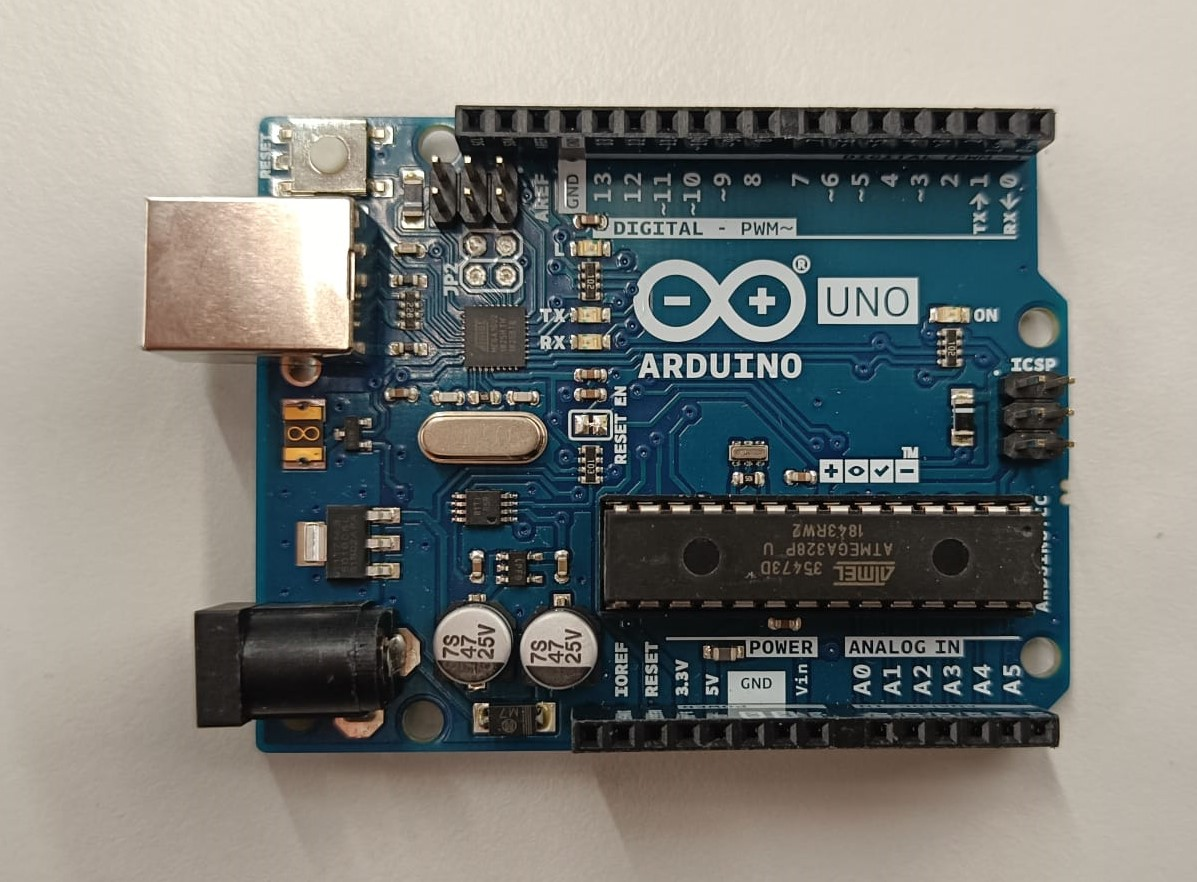
\includegraphics[width=\textwidth]{Arduino_Uno.jpg}
    \caption{Arduino Uno}
  \end{minipage}
  \hfill
  \begin{minipage}[b]{0.4\textwidth}
    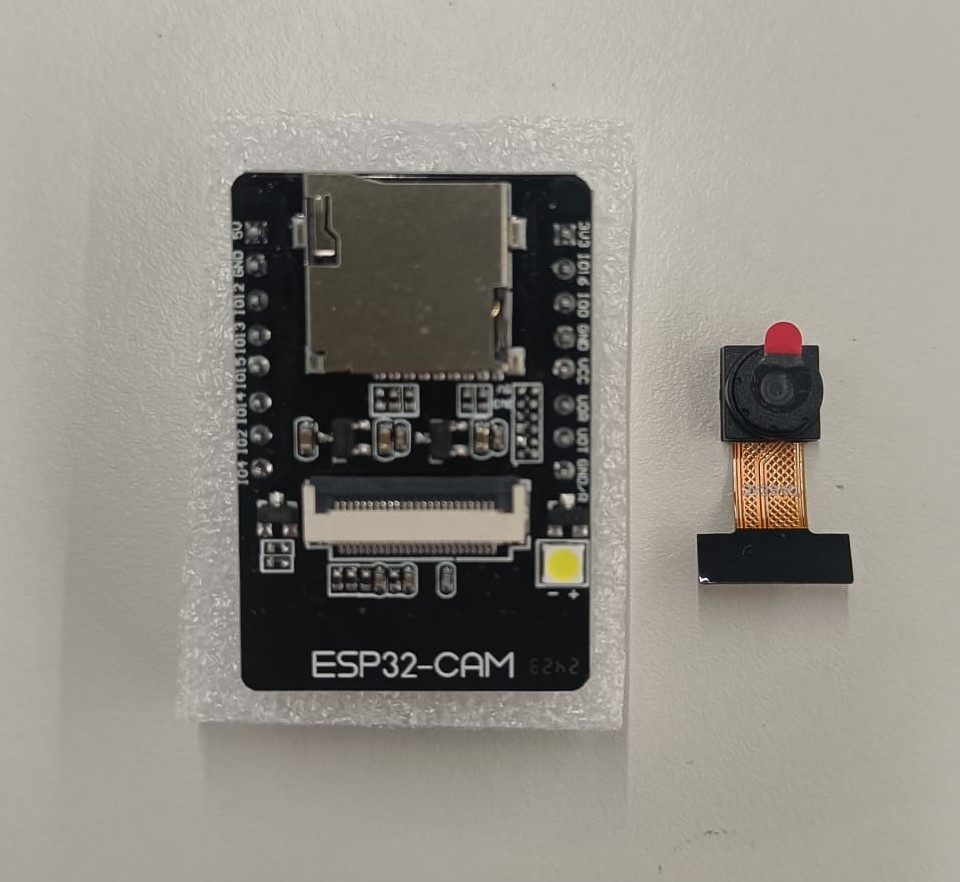
\includegraphics[width=\textwidth]{ESP32_cam.jpg}
    \caption{ESP32-CAM}
  \end{minipage}
\end{figure}

\begin{figure}[H]
  \centering
  \begin{minipage}[b]{0.4\textwidth}
    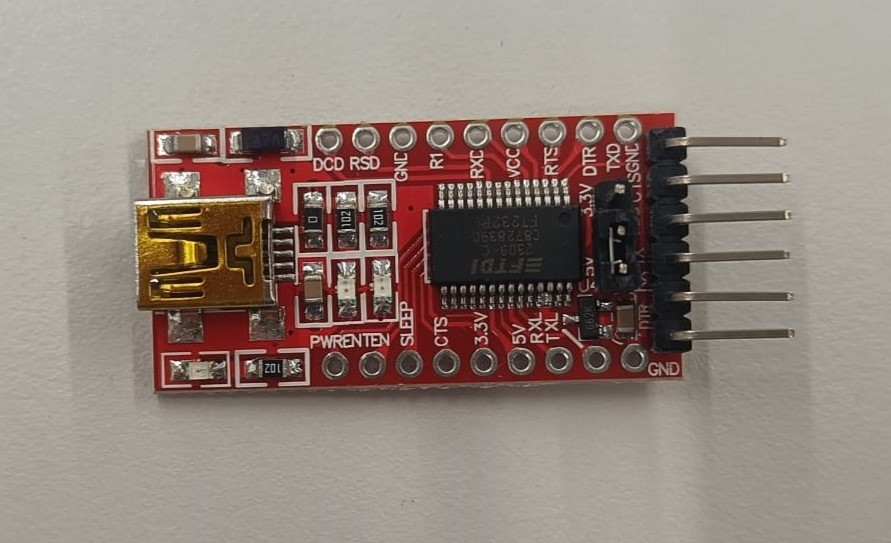
\includegraphics[width=\textwidth]{programmer.jpg}
    \caption{FTDI Programmer}
  \end{minipage}
  \hfill
  \begin{minipage}[b]{0.4\textwidth}
    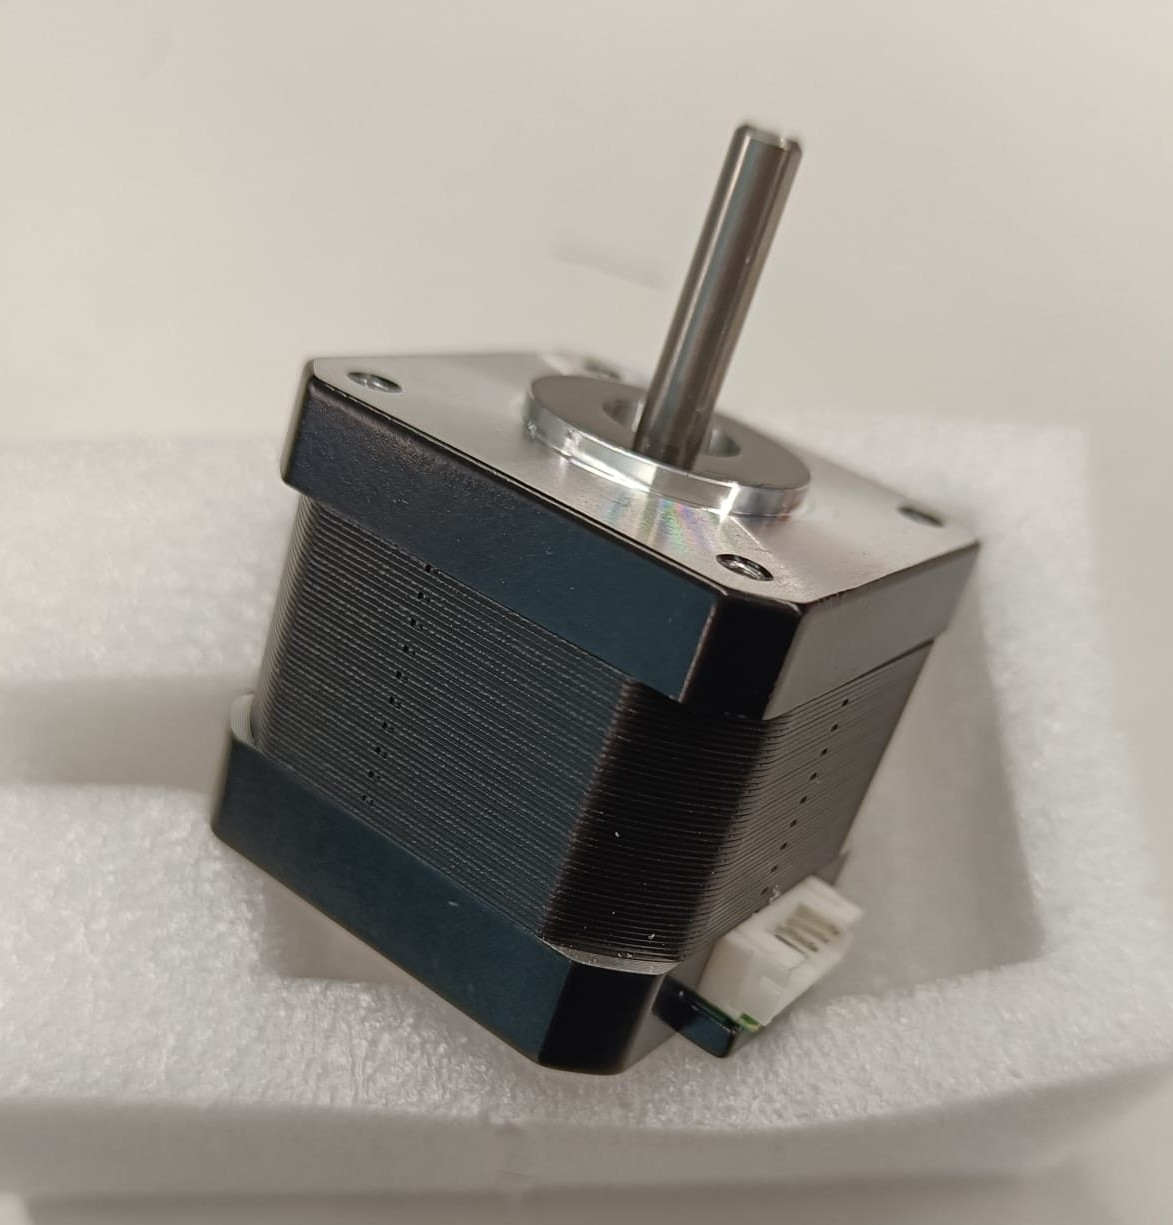
\includegraphics[width=\textwidth]{stepperMotor.jpg}
    \caption{Stepper Motor}
  \end{minipage}
\end{figure}

\begin{figure}[H]
  \centering
  \begin{minipage}[b]{0.4\textwidth}
    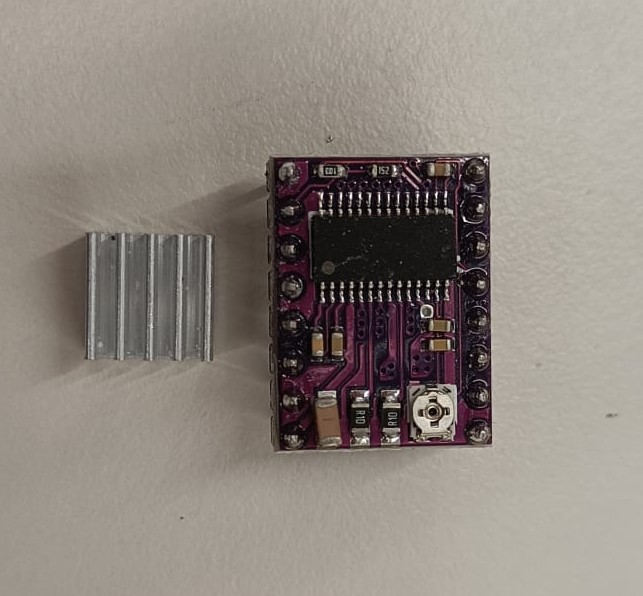
\includegraphics[width=\textwidth]{driver.jpg}
    \caption{Driver for the motor}
  \end{minipage}
  \hfill
  \begin{minipage}[b]{0.4\textwidth}
    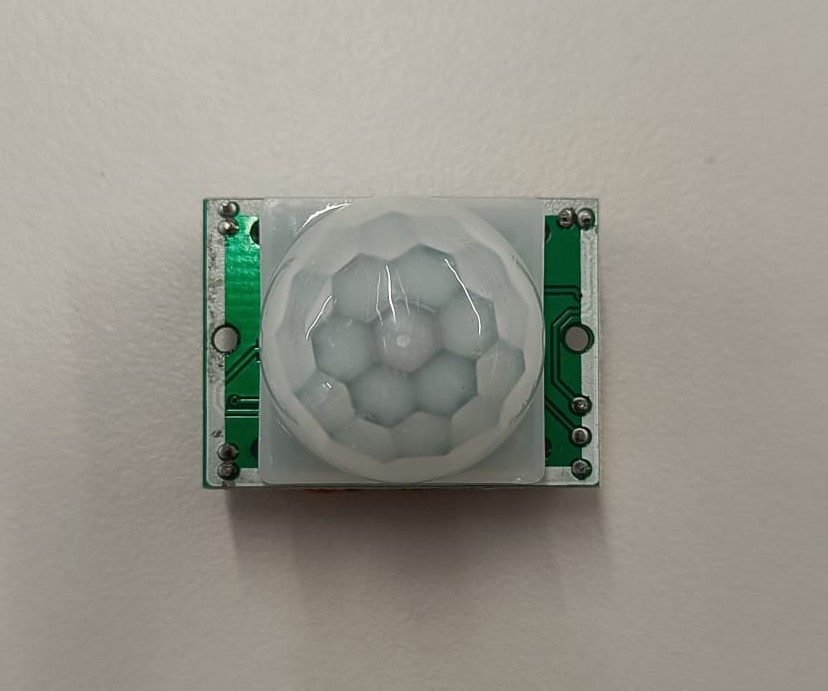
\includegraphics[width=\textwidth]{sensor.jpg}
    \caption{Motion Sensors}
  \end{minipage}
\end{figure}


\newpage
\section{Assembly and programming}

\subsection{Programming of the ESP32-CAM}
First, the camera module needs to be programmed in such a way that it takes a picture upon input from the Arduino and saves it on the inserted MicroSD card. \\
Initially, we followed the commonly recommended approach to use the deep-sleep functionality of the ESP32-CAM \cite{esp_cam_start}. This would wake up the camera whenever a high signal is detected on a specified pin. However, we found that only pins on the left side of the board can be used for that, which came with the problem that most pins of the ESP32-CAM are also used for internal functionality, such as writing to the SD card \cite{esp_cam_pins}. We were able to be partially fix this by mounting the card in 1-bit mode, which enables you to use pin 13 for the wake-up. But since the flash and SD card internally both use pin 4, the flash would not work anymore when we tried this approach. \\
Therefore, we decided to not use the deep-sleep of the ESP32-CAM and instead take the pictures in its loop function \cite{esp_cam_loop}.
With that we can constantly listen to the signal on pin 1, which is normally used for serial communication. Since we do not depend on that after uploading the code, this allowed us to use the SD card while also having the flash enabled. \\
Our final code can be found on our GitHub repository \cite{github}.

\subsection{Movement sensors and stepper motor}

The next step is to connect the stepper motor and the motion sensors to the Arduino and get the motor to move in direction of the sensors once they detect movement. \\
For connecting and controlling the stepper motor with the Arduino we mainly referenced the Video on "Stepper Motors and Arduino - The Ultimate Guide" on YouTube \cite{motor_video}. We first made sure that we were able to move the motor as desired without the sensor inputs. This was quite the challenge, since the motor did not always move as programmed but instead quite unpredictably. We think the problem arose from the power supply and we ultimately tried to fix it by adding a second capacitor between the power cable and the driver. This helped, but did not fix all motor related problems completely. When initially connecting the motor to the power supply, it sometimes turns quickly without input. It also sometimes misses a few steps. We still don't know why that is and how to fix it.\\
For connecting the motion sensor we first followed the article on "How to Use a PIR Motion Sensor With Arduino" by Autodesk Instructables \cite{motio_sensor_guide}. We then placed the two sensors on both sides of the motor with the motor pointing to the middle. Every time one of the sensors picked up a movement, we programmed the motor to move in its direction, wait for a second and then move back to its original position. If both sensors detect a movement, the camera stays in its initial position. We also adjusted the sensitivity of the sensors to our liking. Ultimately, the Arduino will send an input to the camera module during the waiting period to take the picture before moving back into position. The code for the Arduino can also be found on our GitHub repository \cite{github}. 

\subsection{Connecting everything together} 
At the end, all the parts need to be assembled as shown here:\\
\\
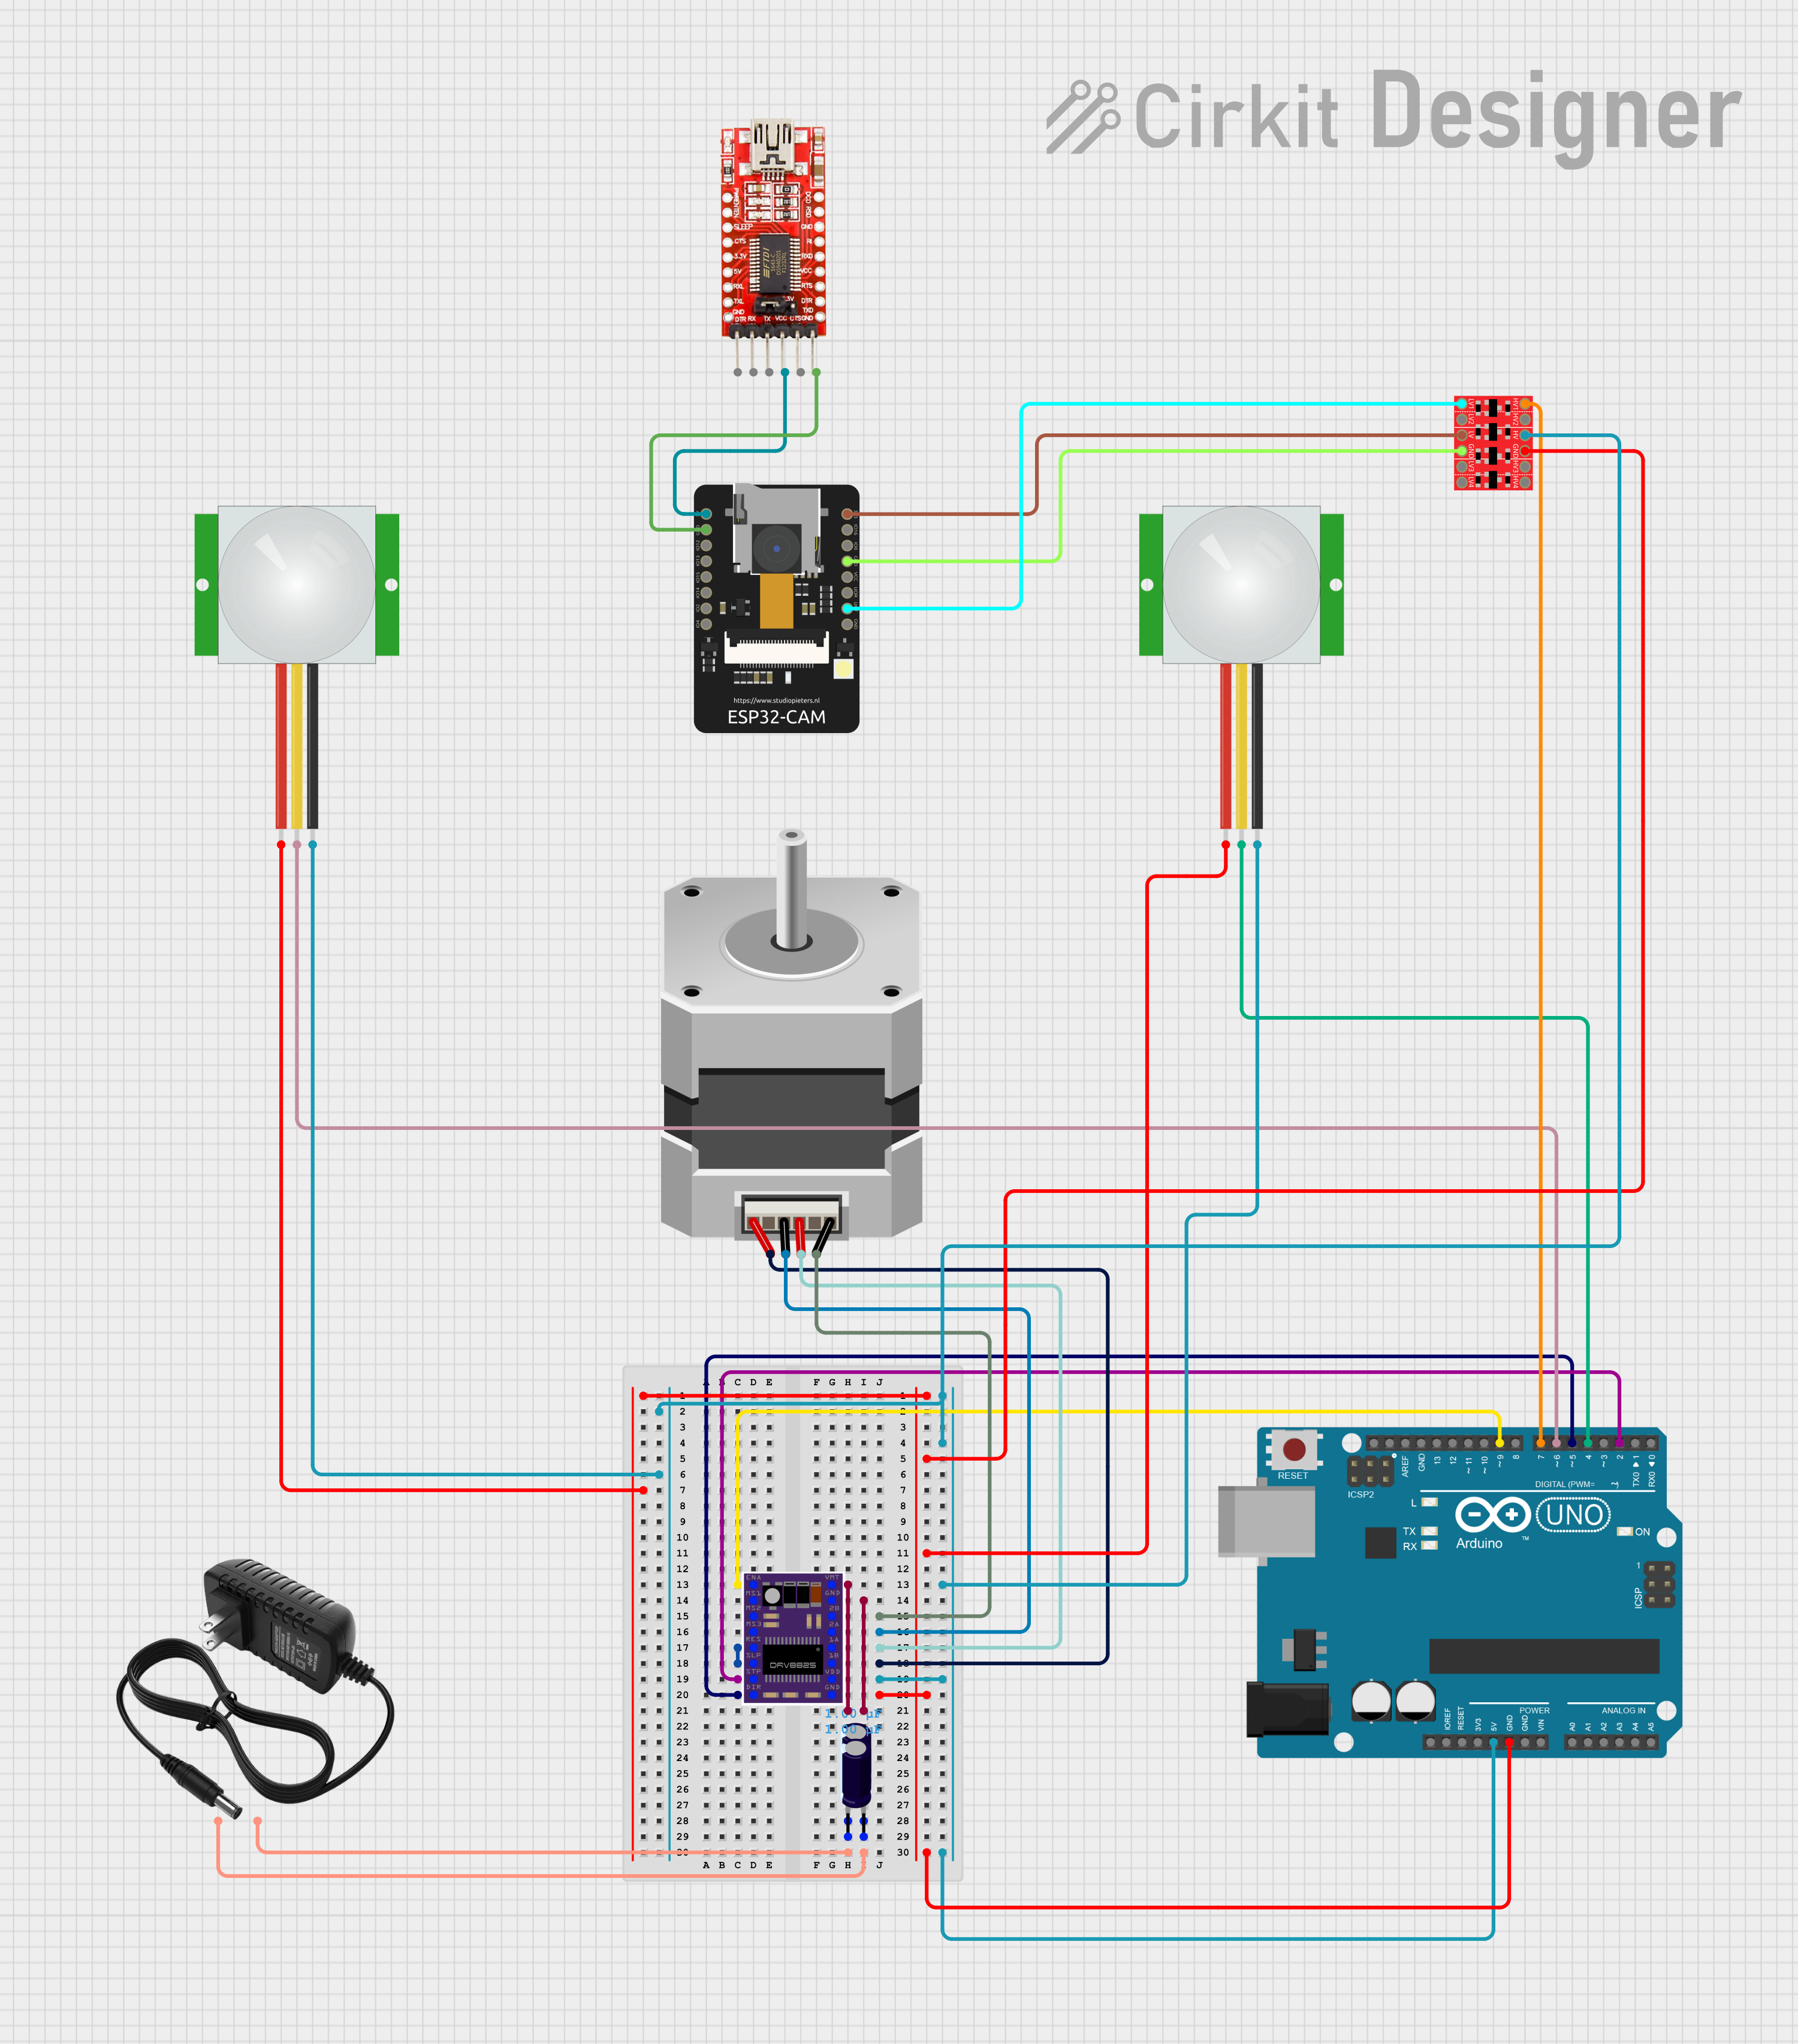
\includegraphics[width=\textwidth]{circuit_image(1).png}

\newpage
\section{Conclusion and lessons learned}
\subsection{Divison of labor}
At the beginning, we mostly worked as a team and met together to work on the project and discuss further steps.\\
Later, as things got more hectic, we split up into two groups. One, consisting of Heinrich and Simon, working on the camera module. This took a lot longer than anticipated due to problems with saving the pictures to the MicroSD card. The other team, consisting of Lina and Jennifer, started to assemble the motor and motion sensors at the same time. This also presented as a challenge since the motor behaved quite unpredictably at times. On the way to the finished product, not many drivers survived and we learned that capacitors tend to explode when plugged in the wrong way.\\
At the end, we assembled the two separate parts together and all worked on the finishing touches as well as this report and the presentation.

\subsection{Critical self-assessment}
The main aspect that we would do differently the next time would be to plan more time for mistakes and to better inform ourselves in advance. We had to order new hardware parts multiple times during the building process, which coast us time, nerves and money. This was because we only realized while stating to build the hardware together, that our parts were either not optimal or that we had forgotten key aspects like the power supply for the stepper motor. This could have been avoided with better planning and initial research to compensate for our lack of knowledge about electronics.\\
Furthermore, we still don't fully now what goes wrong with our motor. We tried to fix the problem with multiple hardware and software approaches which only partly helped.\\
We are however quite proud of ourselves for solving the problem relating the camera module and MicroSD card.

\subsection{Conclusions}
All in all we are very happy with what we achieved during this project. We managed to build a (mostly) working (although not pretty) moving surveillance camera and learned a lot about electronics, voltages and the Arduino along the way. 

\newpage

\printbibliography

\end{document}
